\section{\points[5] Miscellaneous}
\subsection{\points[1] Memes}
\begin{enumerate}
\item \points[1] Draw a meme, write a joke, or share a fun observation related to course material.
\\~\\
This is a bonus question. You will receive full marks for any good-faith attempt.
\end{enumerate}
\clearpage
%% ============================================================
%% ROB 311 — Final Examination, VERSION 2  (problems only, no preamble)
%% ============================================================
%% Points macro — matches quiz style \points[X]
%% Add to preamble if not already present:
%%   \newcommand{\points}[1]{\textbf{[#1 pts]}}
\subsection{\points[2] Evolutionary Learning}
For each question, circle the single best answer.
\begin{enumerate}
%% ---- MC1: Replicator dynamics ----
\item \points[1] In replicator dynamics, the fraction of the population playing strategy $i$
\emph{declines} when:
\choice[Strategy $i$ is strictly dominated in the underlying normal-form game.] \\
\choice[The population fraction of strategy $i$ is below $1/2$.] \\
\choicecorrect[The payoff to strategy $i$ is below the population-average payoff.] \\
\choice[The payoff to strategy $i$ is below the payoff of the best-performing strategy.]
%% ---- MC2: ESS / Nash ----
\item  \points[1] Which of the following correctly describes the relationship between
evolutionary stable strategies (ESS) and Nash equilibria? \\
\choice[Every Nash equilibrium is an ESS, but not every ESS is a Nash equilibrium.] \\
\choice[ESS and Nash equilibria are exactly the same set.] \\
\choicecorrect[Every ESS is a Nash equilibrium, but not every Nash equilibrium is an ESS.] \\
\choice[A strategy can be an ESS without being a rest point of the replicator dynamics.]
\end{enumerate}
\subsection{\points[2] Learning Theory}
For each question, circle the single best answer.
\begin{enumerate}
%% ---- MC3: PAC learning ----
\item  \points[1] In the PAC learning framework with parameters $(\varepsilon,\delta)$, the
parameter $\delta$ is best described as:\\
\choice[The largest true error the returned hypothesis is allowed to have.] \\
\choice[The fraction of the training examples that the returned hypothesis may misclassify.] \\
\choicecorrect[The largest allowed probability that the returned hypothesis has true error greater than $\varepsilon$.] \\
\choice[The probability that a randomly drawn training example carries an incorrect label.]
%% ---- MC4: Hoeffding's inequality ----
\item  \points[1] In Hoeffding's inequality, holding the number of samples $n$ fixed,
\emph{halving} $\varepsilon$:\\
\choice[Halves the bound on the deviation probability.] \\
\choicecorrect[Weakens the bound, replacing the factor $e^{-2n\varepsilon^2}$ with $e^{-n\varepsilon^2/2}$.] \\
\choice[Strengthens the bound, replacing the factor $e^{-2n\varepsilon^2}$ with $e^{-8n\varepsilon^2}$.] \\
\choice[Has no effect, since the bound depends only on $n$ and the range of the random variables.]
\end{enumerate}
\clearpage
\section{\points[12] Search Problems}
\subsection{\points[12] Algorithm Tracing}
Consider the search problem over the graph below. The cost of each transition is represented by the weight of its associated edge. The heuristic value of each sate is represented in parentheses beside the associated vertex. The initial state is $s_0 = A$ and the goal set is $\mathcal{G} = \{G\}$.
\begin{figure}[H]
\centering
\begin{tikzpicture}[
  auto, semithick,
  every state/.style={draw=black, thick, fill=white, minimum size=7mm}
]
\node[state] (A) at (0, 0)    {$A$};
\node[state] (B) at (-3,-1.5) {$B$};
\node[state] (C) at ( 3,-1.5) {$C$};
\node[state] (E) at (-3,-3.5) {$E$};
\node[state] (D) at ( 3,-3.5) {$D$};
\node[state] (F) at ( 0,-3.5) {$F$};
\node[state] (G) at ( 0,-5.5) {$G$};
\path[->] (A) edge node[above left]  {$6$} (B);
\path[->] (A) edge node[above right] {$1$} (C);
\path[->] (B) edge node[left]  {$3$} (E);
\path[->] (C) edge[bend right] node[above] {$4$} (E);
\path[->] (C) edge node[right] {$2$} (D);
\path[->] (E) edge node[below] {$1$} (F);
\path[->] (D) edge[bend right] node[below] {$2$} (F);
\path[->, bend right=30] (F) edge node[above] {$1$} (D);
\path[->] (E) edge[bend right=15] node[below left] {$6$} (G);
\path[->] (F) edge node[right] {$3$} (G);
\node[above=1mm of A] {$(8)$};
\node[left=1mm  of B] {$(7)$};
\node[right=1mm of C] {$(7)$};
\node[left=1mm  of E] {$(4)$};
\node[right=1mm of D] {$(8)$};
\node[above=1mm of F] {$(3)$};
\node[right=1mm of G] {$(0)$};
\end{tikzpicture}
\end{figure}
\medskip\noindent
For each algorithm, provide the returned path, $p$ as a sequence of states, \texttt{<$\cdot$,$\cdot$,$\cdot$,$\dots$>} and its associated cost, $\textsf{cst}(p)$, or check the appropriate option.
\paragraph{Assumptions:}
\begin{itemize}
  \item when breaking ties, prefer the node whose path would come first alphabetically
  \item cycle checking (where applicable) is performed at \emph{export time} (before a
        successor is added to the open set).
\end{itemize}
\clearpage
\begin{enumerate}
\item \points[2] Breadth-First Search (no cycle checking). \\[5mm]
$p = \left\langle \ansbox[8cm]{A,B,E,G} \right\rangle, \textsf{cst}(p) = \ansbox[3cm]{15}$ \\[5mm]
\choice[The algorithm terminates but does not return a solution.]\\[5mm]
\choice[This algorithm will result in a cycle.]
\item \points[2] Breadth-First Search with inter-path cycle checking. \\[5mm]
$p = \left\langle \ansbox[8cm]{A,B,E,G} \right\rangle, \textsf{cst}(p) = \ansbox[3cm]{15}$ \\[5mm]
\choice[The algorithm terminates but does not return a solution.]\\[5mm]
\choice[This algorithm will result in a cycle.]
\item \points[2] Depth-First Search (no cycle checking). \\[5mm]
$p = \left\langle \ansbox[8cm]{A,B,E,F,D,F,D,...} \right\rangle, \textsf{cst}(p) = \numbox[3cm]$ \\[5mm]
\choice[The algorithm terminates but does not return a solution.]\\[5mm]
\choicecorrect[This algorithm will result in a cycle.]
\clearpage
\item \points[2] Depth-First Search with intra-path cycle checking. \\[5mm]
$p = \left\langle \ansbox[8cm]{A,B,E,F,G} \right\rangle, \textsf{cst}(p) = \ansbox[3cm]{13}$ \\[5mm]
\choice[The algorithm terminates but does not return a solution.]\\[5mm]
\choice[This algorithm will result in a cycle.]
\item \points[2] Cheapest-First (Uniform-Cost) Search. \\[5mm]
$p = \left\langle \ansbox[8cm]{A,C,D,F,G} \right\rangle, \textsf{cst}(p) = \ansbox[3cm]{8}$ \\[5mm]
\choice[The algorithm terminates but does not return a solution.]\\[5mm]
\choice[This algorithm will result in a cycle.]
\item \points[2] A*, using the heuristic values shown. \\[5mm]
$p = \left\langle \ansbox[8cm]{A,C,E,F,G} \right\rangle, \textsf{cst}(p) = \ansbox[3cm]{9}$ \\[5mm]
\choice[The algorithm terminates but does not return a solution.]\\[5mm]
\choice[This algorithm will result in a cycle.]
\begin{solution}
Successors are generated alphabetically:
$A:\{B,C\}$, $B:\{E\}$, $C:\{D,E\}$, $D:\{F\}$, $E:\{F,G\}$, $F:\{D,G\}$.
\medskip
\noindent\textbf{BFS.} Frontier by depth:
$\langle A,B\rangle,\langle A,C\rangle$;
$\langle A,B,E\rangle,\langle A,C,D\rangle,\langle A,C,E\rangle$;
$\langle A,B,E,F\rangle,\langle A,B,E,G\rangle,\dots$
The first goal expanded is $\langle A,B,E,G\rangle$, $\textsf{cst}=6+3+6=15$.
With inter-path cycle checking, $E$ is pruned when generated from $C$ and $F$ is pruned when
generated from $D$, but $\langle A,B,E,G\rangle$ is still the first goal reached, so the answer
is unchanged.
\medskip
\noindent\textbf{DFS.} $A\to B\to E\to F\to D\to F\to D\to\cdots$: the algorithm loops on the
cycle $D\to F\to D$ and never terminates.
With intra-path cycle checking, $D$'s only successor $F$ is already on the path, so the branch
dies and the search backtracks to $\langle A,B,E,F,G\rangle$, $\textsf{cst}=6+3+1+3=13$.
\medskip
\noindent\textbf{Cheapest-first.} Path costs to $G$ are
$\langle A,C,D,F,G\rangle = 8$, $\langle A,C,E,F,G\rangle = 9$, $\langle A,C,E,G\rangle = 11$,
$\langle A,B,E,F,G\rangle = 13$, $\langle A,B,E,G\rangle = 15$.
The cheapest is $\langle A,C,D,F,G\rangle$ with $\textsf{cst}=1+2+2+3=8$.
\medskip
\noindent\textbf{A*.} With $f = g+h$:
$\langle A,C\rangle$ has $f=1+7=8$ and $\langle A,B\rangle$ has $f=6+7=13$, so $C$ is expanded.
Then $\langle A,C,D\rangle$ has $f=3+8=11$ while $\langle A,C,E\rangle$ has $f=5+4=9$, so the
$E$ branch is preferred; $\langle A,C,E,F\rangle$ has $f=6+3=9$ and
$\langle A,C,E,F,G\rangle$ has $f=9$, which is expanded first and returns
$\langle A,C,E,F,G\rangle$, $\textsf{cst}=9$.
\medskip
\noindent Note that $h(D)=8$ overestimates the true cost-to-go from $D$ (which is $5$), so the
heuristic is \emph{inadmissible} and A* returns a suboptimal path here.
\end{solution}
\end{enumerate}
\clearpage
%% ============================================================
\section{\points[16] Probabilistic Inference}
\subsection{\points[8] Dependence Separation}
Consider the Bayesian network below.
\begin{figure}[H]
\centering
\begin{tikzpicture}[
  auto, semithick,
  every state/.style={draw=black, thick, fill=white, minimum size=7mm},
  node distance=1.8cm
]
\node[state] (X) at (-1, 1.5) {$X$};
\node[state] (Y) at ( 1, 1.5) {$Y$};
\node[state] (Z) at ( 0, 0)   {$Z$};
\node[state] (W) at ( 0,-1.5) {$W$};
\node[state] (V) at ( 0,-3.0) {$V$};
\node[state] (U) at ( 2.5, 0) {$U$};
\path[-latex] (X) edge (Z);
\path[-latex] (Y) edge (Z);
\path[-latex] (Z) edge (W);
\path[-latex] (W) edge (V);
\path[-latex] (Y) edge (U);
\end{tikzpicture}
\end{figure}
\noindent
Determine whether each statement is true or false, or indicate that there isn't enough information to determine the answer.
\begin{enumerate}
\item \points[2] $X \perp Y$ \\[5mm]
\choicecorrect[True]\choice[False]\choice[Not enough information]
\item \points[2] $X \perp Y \mid V$ \\[5mm]
\choice[True]\choicecorrect[False]\choice[Not enough information]
\item \points[2] $X \perp U$\\[5mm]
\choicecorrect[True]\choice[False]\choice[Not enough information]
\item \points[2] $X \perp U \mid W$\\[5mm]
\choice[True]\choicecorrect[False]\choice[Not enough information]
\end{enumerate}
\begin{solution}
If students answered "Not enough information" instead of "False", only 1 mark penalty.
\medskip
\noindent (1) The only path is $X \to Z \leftarrow Y$. $Z$ is a collider and neither $Z$ nor any
descendant of $Z$ is observed, so the path is blocked: \textbf{True}.
\noindent (2) $V$ is a descendant of the collider $Z$ (via $Z\to W\to V$), so observing $V$
activates the collider and the path $X \to Z \leftarrow Y$ becomes active: \textbf{False}.
\noindent (3) The only path is $X \to Z \leftarrow Y \to U$. The collider $Z$ is unobserved
with no observed descendant, so the path is blocked: \textbf{True}.
\noindent (4) Conditioning on $W$ (a descendant of $Z$) activates the collider $Z$; $Y$ is a
fork on the path and is not observed, so the path $X \to Z \leftarrow Y \to U$ is active:
\textbf{False}.
\end{solution}
\clearpage
\subsection{\points[8] Exact Inference via Bayes' Rule}
Consider the Bayesian network below, where $A, B, C, D$ are binary random variables over
$\{0,1\}$.
\begin{figure}[H]
\centering
\begin{tikzpicture}[
  auto, semithick,
  every state/.style={draw=black, thick, fill=white, minimum size=7mm}
]
\node[state] (A) at ( 0,  0)   {$A$};
\node[state] (B) at (-2, -1.5) {$B$};
\node[state] (C) at (-4, -3)   {$C$};
\node[state] (D) at ( 2, -3)   {$D$};
\path[-latex] (A) edge (B);
\path[-latex] (B) edge (C);
\path[-latex] (A) edge (D);
\path[-latex] (C) edge (D);
\end{tikzpicture}
\end{figure}
\noindent The conditional probability tables are:
\begin{table}[H]
\centering
\begin{tabular}{|c|c|}
\hline
$A$ & $P(A=1)$ \\\hline
    & $0.25$   \\\hline
\end{tabular}
\hspace{8mm}
\begin{tabular}{|c|c|}
\hline
$A$ & $P(B=1\mid A)$ \\\hline
$0$ & $0.2$          \\\hline
$1$ & $0.6$          \\\hline
\end{tabular}
\hspace{8mm}
\begin{tabular}{|c|c|}
\hline
$B$ & $P(C=1\mid B)$ \\\hline
$0$ & $0.1$          \\\hline
$1$ & $0.6$          \\\hline
\end{tabular}
\end{table}
\begin{table}[H]
\centering
\begin{tabular}{|c|c|c|}
\hline
$A$ & $C$ & $P(D=1\mid A,C)$ \\\hline
$0$ & $0$ & $0.20$           \\\hline
$0$ & $1$ & $0.40$           \\\hline
$1$ & $0$ & $0.50$           \\\hline
$1$ & $1$ & $0.90$           \\\hline
\end{tabular}
\end{table}
\begin{enumerate}
\item \points[8] Find the exact value of $P(A=1 \mid D=1)$. Provide your answer in fractional form.  Show your work. \\[5mm]
$\textsf{pr}(A=1|D=1) = \ansbox[3cm]{11} \; \Bigg/ \; \ansbox[3cm]{23}$\vspace{180pt}
\begin{solution}
By Bayes' rule:
\[
  P(A=1\mid D=1) = \frac{P(D=1\mid A=1)\,P(A=1)}{P(D=1)}.
\]
We marginalize over $B$ to compute $P(C=1\mid A)$:
\begin{align*}
  P(C=1\mid A=0) &= P(C=1\mid B=0)\,P(B=0\mid A=0) + P(C=1\mid B=1)\,P(B=1\mid A=0) \\
                 &= 0.1 \times 0.8 + 0.6 \times 0.2 = 0.08 + 0.12 = 0.20,\\[4pt]
  P(C=1\mid A=1) &= P(C=1\mid B=0)\,P(B=0\mid A=1) + P(C=1\mid B=1)\,P(B=1\mid A=1) \\
                 &= 0.1 \times 0.4 + 0.6 \times 0.6 = 0.04 + 0.36 = 0.40.
\end{align*}
Hence:
\[
  P(C=0\mid A=0)=1-0.20=0.80,\qquad P(C=0\mid A=1)=1-0.40=0.60.
\]
Now marginalize over $C$ to compute $P(D=1\mid A)$:
\begin{align*}
  P(D=1\mid A=0) &= P(D=1\mid A=0,C=0)\,P(C=0\mid A=0) \\
  &+ P(D=1\mid A=0,C=1)\,P(C=1\mid A=0) \\
                 &= 0.20 \times 0.80 + 0.40 \times 0.20 = 0.16 + 0.08 = 0.24,\\[4pt]
  P(D=1\mid A=1) &= P(D=1\mid A=1,C=0)\,P(C=0\mid A=1) \\
  &+ P(D=1\mid A=1,C=1)\,P(C=1\mid A=1) \\
                 &= 0.50 \times 0.60 + 0.90 \times 0.40 = 0.30 + 0.36 = 0.66.
\end{align*}
Then:
\[
  P(D=1) = P(D=1\mid A=0)\,P(A=0) + P(D=1\mid A=1)\,P(A=1)
         = 0.24\times 0.75 + 0.66\times 0.25
\]
\[
  = 0.180 + 0.165 = 0.345.
\]
Therefore:
\[
  P(A=1\mid D=1) = \frac{0.66 \times 0.25}{0.345} = \frac{0.165}{0.345} = \frac{11}{23} \approx 0.4783.
\]
\end{solution}
\end{enumerate}
\clearpage
\begin{center}
    \textit{(extra space)}
\end{center}
\clearpage
%% ============================================================
\section{\points[18] Markov Decision Processes}
\subsection{\points[12] Q-Value Iteration}
Consider an MDP with $\mathcal{S} = \{s_1, s_2, s_3\}$ and
$\mathcal{A} = \{\texttt{A},\texttt{B},\texttt{C}\}$.
Transitions and rewards are shown in the diagram below.
\begin{figure}[H]
\vspace{15pt}
\centering
\begin{tikzpicture}[
  auto, semithick,
  every state/.style={draw=black, thick, fill=white, minimum size=10mm}
]
%======================
% States
%======================
\node[state] (s1) at (0,3.5)  {$s_1$};
\node[state] (s2) at (6,3.5)  {$s_2$};
\node[state] (s3) at (12,3.5) {$s_3$};
%======================
% Actions
%======================
\node[state, dashed] (a1A) at (-1,0) {\texttt{A}};
\node[state, dashed] (a1B) at (0,0)  {\texttt{B}};
\node[state, dashed] (a1C) at (1,0)  {\texttt{C}};
\node[state, dashed] (a2A) at (5,7)  {\texttt{A}};
\node[state, dashed] (a2B) at (6,7)  {\texttt{B}};
\node[state, dashed] (a2C) at (7,7)  {\texttt{C}};
\node[state, dashed] (a3A) at (11,0) {\texttt{A}};
\node[state, dashed] (a3B) at (12,0) {\texttt{B}};
\node[state, dashed] (a3C) at (13,0) {\texttt{C}};
%======================
% State -> Action
%======================
\path[-latex, dashed] (s1) edge (a1A);
\path[-latex, dashed] (s1) edge (a1B);
\path[-latex, dashed] (s1) edge (a1C);
\path[-latex, dashed] (s2) edge (a2A);
\path[-latex, dashed] (s2) edge (a2B);
\path[-latex, dashed] (s2) edge (a2C);
\path[-latex, dashed] (s3) edge (a3A);
\path[-latex, dashed] (s3) edge (a3B);
\path[-latex, dashed] (s3) edge (a3C);
%======================
% Transitions
%======================
% s1
\path[-latex, overlay] (a1A) edge[out=110, in=100, looseness=1.4]
  node[pos=0.5, font=\small, fill=white, above=2mm] {$+2$} (s3);
\path[-latex] (a1B) edge[bend left=30] node[pos=0.5, font=\small, fill=white] {$+1$} (s2);
\path[-latex] (a1C) edge[bend left=10]  node[pos=0.5, font=\small, fill=white] {$+3$} (s2);
\path[-latex] (a1C) edge[bend right=30] node[above=5mm, pos=0.3, font=\small, fill=white] {$+3$} (s3);
% s2
\path[-latex] (a2A) edge[bend right=20] node[pos=0.5, font=\small, fill=white] {$+4$} (s1);
\path[-latex] (a2B) edge[bend right=10] node[pos=0.5, font=\small, fill=white] {$+2$} (s3);
\path[-latex] (a2C) edge[bend left=10]  node[pos=0.5, font=\small, fill=white] {$+1$} (s1);
\path[-latex] (a2C) edge[bend left=20]  node[pos=0.5, font=\small, fill=white] {$+5$} (s3);
% s3
\path[-latex] (a3A) edge[bend left=30]  node[below=5mm, pos=0.5, font=\small, fill=white] {$+1$} (s1);
\path[-latex] (a3A) edge[bend right=10] node[pos=0.5, font=\small, fill=white] {$+3$} (s2);
\path[-latex] (a3B) edge[loop below] node[pos=0.5, font=\small, fill=white] {$+2$} (a3B);
\path[-latex] (a3C) edge[bend right=30] node[pos=0.5, font=\small, fill=white] {$+4$} (s2);
\end{tikzpicture}
\end{figure}
\paragraph{Assumptions.}
\begin{itemize}
  \item $p(s'\mid s,a)$ is uniform over all successors shown from the action node.
  \item Discount factor $\gamma = 0.9$; time horizon $T = 2$.
  \item Initial Q-values: $q(s,a;\,2) \equiv 0$ for all $s \in \mathcal{S}$, $a \in \mathcal{A}$.
  \item All Q-values are updated synchronously via
  \[
    q(s,a;\,t) = \sum_{s'} p(s'\mid s,a)\Bigl[r(s,a,s') + \gamma\max_{a'}q(s',a';\,t+1)\Bigr].
  \]
\end{itemize}
\begin{enumerate}
\clearpage
\item \points[8] Fill in the Q-value tables below.
\renewcommand{\arraystretch}{1.9}
\begin{table}[H]
\centering
\begin{tabular}{|c|c|c|c|c|c|}
\hline
$s$ & $a$ & $q(s,a;\,2)$ & $q(s,a;\,1)$ & $q(s,a;\,0)$ & $\pi^*(a|s)$\\\hline
$s_1$ & \texttt{A} & $0$ & \ansnt{$2$}    & \ansnt{$5.60$} & \ansnt{$0$} \\\hline
$s_1$ & \texttt{B} & $0$ & \ansnt{$1$}    & \ansnt{$4.60$} & \ansnt{$0$} \\\hline
$s_1$ & \texttt{C} & $0$ & \ansnt{$3$}    & \ansnt{$6.60$} & \ansnt{$1$} \\\hline
$s_2$ & \texttt{A} & $0$ & \ansnt{$4$}    & \ansnt{$6.70$} & \ansnt{$1$} \\\hline
$s_2$ & \texttt{B} & $0$ & \ansnt{$2$}    & \ansnt{$5.60$} & \ansnt{$0$} \\\hline
$s_2$ & \texttt{C} & $0$ & \ansnt{$3$}    & \ansnt{$6.15$} & \ansnt{$0$} \\\hline
$s_3$ & \texttt{A} & $0$ & \ansnt{$2$}    & \ansnt{$5.15$} & \ansnt{$0$} \\\hline
$s_3$ & \texttt{B} & $0$ & \ansnt{$2$}    & \ansnt{$5.60$} & \ansnt{$0$} \\\hline
$s_3$ & \texttt{C} & $0$ & \ansnt{$4$}    & \ansnt{$7.60$} & \ansnt{$1$} \\\hline
\end{tabular}
\end{table}
\begin{solution}
At $t=1$ the Q-values are just expected immediate rewards:
\[
q(s_1,\texttt{C};1)=\tfrac12(3)+\tfrac12(3)=3,\quad
q(s_2,\texttt{C};1)=\tfrac12(1)+\tfrac12(5)=3,\quad
q(s_3,\texttt{A};1)=\tfrac12(1)+\tfrac12(3)=2,
\]
and the remaining (deterministic) actions inherit their listed rewards. Hence
\[
\max_{a}q(s_1,a;1)=3,\qquad \max_{a}q(s_2,a;1)=4,\qquad \max_{a}q(s_3,a;1)=4.
\]
At $t=0$, with $\gamma=0.9$:
\begin{align*}
q(s_1,\texttt{A};0)&=2+0.9(4)=5.60, &
q(s_1,\texttt{B};0)&=1+0.9(4)=4.60, \\
q(s_1,\texttt{C};0)&=\tfrac12\bigl[3+0.9(4)\bigr]+\tfrac12\bigl[3+0.9(4)\bigr]=6.60, &
q(s_2,\texttt{A};0)&=4+0.9(3)=6.70, \\
q(s_2,\texttt{B};0)&=2+0.9(4)=5.60, &
q(s_2,\texttt{C};0)&=\tfrac12\bigl[1+0.9(3)\bigr]+\tfrac12\bigl[5+0.9(4)\bigr]=6.15, \\
q(s_3,\texttt{A};0)&=\tfrac12\bigl[1+0.9(3)\bigr]+\tfrac12\bigl[3+0.9(4)\bigr]=5.15, &
q(s_3,\texttt{B};0)&=2+0.9(4)=5.60, \\
q(s_3,\texttt{C};0)&=4+0.9(4)=7.60. &&
\end{align*}
\end{solution}
\item \points[2] Identify the greedy policy $\pi(a\mid s)$ derived from $q(s,a;\,0)$
for each $s \in \mathcal{S}$ and provide it in the table above.
\begin{solution}
$\texttt{C}$ at $s_1$, $\texttt{A}$ at $s_2$, and $\texttt{C}$ at $s_3$.
\end{solution}
\item \points[2] Without further computation, explain what happens to the greedy policy as $\gamma \to 0$.
\begin{solution}
As $\gamma \to 0$, future rewards are ignored, so the greedy policy approaches the policy that chooses the action with the largest expected \emph{immediate} reward at each state, i.e.\ the greedy policy with respect to the $q(s,a;1)$ column. For this MDP that column is maximised by \texttt{C} at $s_1$, \texttt{A} at $s_2$, and \texttt{C} at $s_3$, so the greedy policy is unchanged.
\end{solution}
\vspace{60pt}
\end{enumerate}
\clearpage
\subsection{\points[6] State Estimation in Partially Observable MDPs}
Consider the same MDP structure with $\mathcal{S}=\{s_1,s_2,s_3\}$ and
$\mathcal{A}=\{\texttt{A},\texttt{B},\texttt{C}\}$.
The transition probabilities under action \texttt{B} are:
\[
p(s_2\mid s_1,\texttt{B})=1,\quad
p(s_2\mid s_2,\texttt{B})=0.5,\quad
p(s_3\mid s_2,\texttt{B})=0.5,\quad
p(s_3\mid s_3,\texttt{B})=1.
\]
The observation model is:
\[
m(o\mid s) = \begin{cases} 0.7 & o = s \\ 0.15 & o \neq s \end{cases}
\]
for each of the other two states.
\begin{enumerate}
\item \points[6] The prior belief is $b(s_1)=0.4$,\; $b(s_2)=0.4$,\; $b(s_3)=0.2$.
The agent takes action $\texttt{B}$ and receives observation $o = s_2$.
Compute the posterior belief $b(s \mid a=\texttt{B},\, o=s_2)$.
\renewcommand{\arraystretch}{2.4}
\setlength{\tabcolsep}{18pt}   % default is 6pt
\begin{table}[H]
\centering
\begin{tabular}{|c|c|c|c|}
\hline
$s$ & $s_1$ & $s_2$ & $s_3$ \\\hline
$b(s)$ & $0.4$ & $0.4$ & $0.2$ \\\hline
$b(s \mid a=\texttt{B},\, o=s_2)$ &
\ansnt{$0$} & \ansnt{$0.875$} & \ansnt{$0.125$} \\\hline
\end{tabular}
\end{table}
\begin{solution}
\textbf{Step 1: Predict} (propagate belief through action $\texttt{B}$).
\begin{align*}
  b'(s_1) &= b(s_1)\,p(s_1\mid s_1,\texttt{B}) + b(s_2)\,p(s_1\mid s_2,\texttt{B}) + b(s_3)\,p(s_1\mid s_3,\texttt{B}) \\
           &= 0 + 0 + 0 = 0, \\[4pt]
  b'(s_2) &= b(s_1)\,p(s_2\mid s_1,\texttt{B}) + b(s_2)\,p(s_2\mid s_2,\texttt{B}) + b(s_3)\,p(s_2\mid s_3,\texttt{B}) \\
           &= 0.4\times 1 + 0.4\times 0.5 + 0 = 0.4 + 0.2 = 0.6, \\[4pt]
  b'(s_3) &= b(s_1)\,p(s_3\mid s_1,\texttt{B}) + b(s_2)\,p(s_3\mid s_2,\texttt{B}) + b(s_3)\,p(s_3\mid s_3,\texttt{B}) \\
           &= 0 + 0.4\times 0.5 + 0.2\times 1 = 0.2 + 0.2 = 0.4.
\end{align*}
\medskip
\noindent\textbf{Step 2: Update} (condition on observation $o = s_2$).
\[
  b(s \mid a=\texttt{B}, o=s_2) \propto m(o=s_2 \mid s)\cdot b'(s).
\]
\begin{align*}
  m(s_2 \mid s_1)\cdot b'(s_1) &= 0.15 \times 0 = 0, \\
  m(s_2 \mid s_2)\cdot b'(s_2) &= 0.7 \times 0.6 = 0.42, \\
  m(s_2 \mid s_3)\cdot b'(s_3) &= 0.15 \times 0.4 = 0.06.
\end{align*}
Normaliser: $0 + 0.42 + 0.06 = 0.48$.
\[
  b(s_1 \mid a=\texttt{B}, o=s_2) = 0,\quad
  b(s_2 \mid a=\texttt{B}, o=s_2) = \frac{0.42}{0.48} = 0.875,\quad
  b(s_3 \mid a=\texttt{B}, o=s_2) = \frac{0.06}{0.48} = 0.125.
\]
Note that here the update step \emph{does} change the relative proportions: the observation
matches $s_2$ but not $s_3$, so those two states are re-weighted by different likelihoods
($0.7$ versus $0.15$).
\end{solution}
\vspace{120pt}
\end{enumerate}
\clearpage
\begin{center}
    \textit{(extra space)}
\end{center}
\clearpage
%% ============================================================
\section{\points[20] Normal-Form Games}
\subsection{\points[8] Pure and Mixed Nash Equilibria}
Consider the following 2-player normal-form game.
\begin{table}[H]
\centering
\begin{tabular}{|c|c|c|}
\hline
              & $\texttt{L}$    & $\texttt{R}$    \\\hline
$\texttt{T}$  & $(4,\,2)$ & $(1,\,1)$ \\\hline
$\texttt{B}$  & $(0,\,0)$ & $(3,\,5)$ \\\hline
\end{tabular}
\end{table}
\begin{enumerate}
\item \points[3] Identify \emph{all} pure Nash equilibria, or state that none exist.
\\~\\
\checkboxcorrect[(\texttt{L},\texttt{T})]\checkbox[(\texttt{L},\texttt{B})]\checkbox[(\texttt{R},\texttt{T})]\checkboxcorrect[(\texttt{R},\texttt{B})]\choice[No pure equilibrium exists]
\vspace{100pt}
\item \points[5] Find the mixed Nash equilibrium strategy profile
\[
\pi = \bigl((p,\,1-p),\,(q,\,1-q)\bigr),
\]
where $p = \textsf{pr}[\texttt{T}]$ and $q = \textsf{pr}[\texttt{L}]$. Determine whether the mixed
equilibrium is \textbf{stable} or \textbf{unstable} under best-response dynamics, assuming
Agent~1 makes the first update.  Show your work.
\medskip
$p = \ansbox[3cm]{$\frac{5}{6}$}, \quad q = \ansbox[3cm]{$\frac{1}{3}$}$ \medskip \\
The equilibrium is \raisebox{1.75mm}{\choice[stable]} / \raisebox{1.75mm}{\choicecorrect[unstable]} under best-response play.
\begin{solution}
For the mixed Nash equilibrium, let $p=\textsf{pr}[\texttt{T}]$ and $q=\textsf{pr}[\texttt{L}]$.
Agent 1 is indifferent when
\[
4q + 1(1-q) = 0\cdot q + 3(1-q).
\]
Thus,
\[
3q + 1 = 3 - 3q \;\Rightarrow\; 6q = 2 \;\Rightarrow\; q=\frac{1}{3}.
\]
Agent 2 is indifferent when
\[
2p + 0(1-p) = 1\cdot p + 5(1-p).
\]
Thus,
\[
2p = 5 - 4p \;\Rightarrow\; 6p = 5 \;\Rightarrow\; p=\frac{5}{6}.
\]
Therefore, the mixed Nash equilibrium is
\[
\pi = \left(\left(\frac{5}{6},\,\frac{1}{6}\right),\left(\frac{1}{3},\,\frac{2}{3}\right)\right).
\]
This mixed equilibrium is \textbf{unstable} under best-response dynamics. A small deviation causes best responses to push play toward one of the two pure equilibria, $(\texttt{T},\texttt{L})$ or $(\texttt{B},\texttt{R})$, rather than back to the mixed equilibrium.
\end{solution}
\vspace{120pt}
\end{enumerate}
\clearpage
\begin{center}
    \textit{(extra space)}
\end{center}
\clearpage
\subsection{\points[12] Subgame Perfect Equilibria}
Consider a 2-player, 2-stage normal-form game with the following payoff matrices.
\begin{table}[H]
\begin{minipage}{.5\linewidth}
\centering
\begin{tabular}{|c|c|c|}
\hline
             & $\texttt{c}$       & $\texttt{d}$       \\\hline
$\texttt{c}$ & $(3,\,3)$ & $(0,\,5)$ \\\hline
$\texttt{d}$ & $(5,\,0)$ & $(1,\,1)$ \\\hline
\end{tabular}
\caption*{Stage 1}
\end{minipage}%
\begin{minipage}{.5\linewidth}
\centering
\begin{tabular}{|c|c|c|}
\hline
             & $\texttt{e}$       & $\texttt{f}$       \\\hline
$\texttt{e}$ & $(6,\,6)$ & $(1,\,2)$ \\\hline
$\texttt{f}$ & $(2,\,1)$ & $(3,\,3)$ \\\hline
\end{tabular}
\caption*{Stage 2}
\end{minipage}
\end{table}
\noindent Consider the following strategy profile:
\begin{itemize}
  \item Stage 1: each agent plays $\texttt{c}$.
  \item Stage 2: each agent plays $\texttt{e}$ if the Stage-1 outcome was
        $(\texttt{c},\texttt{c})$; otherwise each agent plays $\texttt{f}$.
\end{itemize}
\begin{enumerate}
\item \points[4] Fill in the table below for each possible Stage-1 outcome ($\gamma = 1$).
\renewcommand{\arraystretch}{2.2}
\begin{table}[H]
\centering
\begin{tabular}{|c|c|c|c|c|}
\hline
Stage-1 outcome & Stage-1 rewards & Stage-2 outcome & Stage-2 rewards & Total returns \\\hline
$(\texttt{c},\texttt{c})$ & \ansnt{$(3,\,3)$} & \ansnt{$(\texttt{e},\texttt{e})$} & \ansnt{$(6,\,6)$} & \ansnt{$(9,\,9)$} \\\hline
$(\texttt{d},\texttt{d})$ & \ansnt{$(1,\,1)$} & \ansnt{$(\texttt{f},\texttt{f})$} & \ansnt{$(3,\,3)$} & \ansnt{$(4,\,4)$} \\\hline
$(\texttt{c},\texttt{d})$ & \ansnt{$(0,\,5)$} & \ansnt{$(\texttt{f},\texttt{f})$} & \ansnt{$(3,\,3)$} & \ansnt{$(3,\,8)$} \\\hline
$(\texttt{d},\texttt{c})$ & \ansnt{$(5,\,0)$} & \ansnt{$(\texttt{f},\texttt{f})$} & \ansnt{$(3,\,3)$} & \ansnt{$(8,\,3)$} \\\hline
\end{tabular}
\end{table}
\clearpage
\item \points[4] Is this strategy profile a Nash equilibrium of the 2-stage game?
Justify your answer.
\\~\\
\choicecorrect[Yes]\choice[No]
\begin{solution}
Given the specified continuation strategies, the total returns from Stage 1 are:
\[
(\texttt{c},\texttt{c}) \mapsto (9,9),\quad
(\texttt{d},\texttt{d}) \mapsto (4,4),\quad
(\texttt{c},\texttt{d}) \mapsto (3,8),\quad
(\texttt{d},\texttt{c}) \mapsto (8,3).
\]
Thus, if one player chooses $\texttt{c}$, the other prefers $\texttt{c}$ since $9>8$, and if one player chooses $\texttt{d}$, the other prefers $\texttt{d}$ since $4>3$. Therefore $(\texttt{c},\texttt{c})$ is a Nash equilibrium of the 2-stage game.
Note that the one-shot Stage-1 game is a prisoner's dilemma in which $\texttt{d}$ strictly dominates; it is the threat of reverting to the worse Stage-2 equilibrium $(\texttt{f},\texttt{f})$ that makes cooperation sustainable here, and the margin is exactly $9-8=1$.
\end{solution}
\vspace{160pt}
\item \points[4] Is this strategy profile a subgame perfect equilibrium?
Justify your answer.
\\~\\
\choicecorrect[Yes]\choice[No]
\begin{solution}
After every possible Stage-1 outcome, the prescribed Stage-2 action profile is a Nash equilibrium of the Stage-2 game:
\[
(\texttt{e},\texttt{e}) \text{ is a Nash equilibrium } (6>2), \text{ and } (\texttt{f},\texttt{f}) \text{ is also a Nash equilibrium } (3>1).
\]
Moreover, at Stage 1, given these continuation payoffs, $(\texttt{c},\texttt{c})$ is a Nash equilibrium. Hence the strategy profile is a subgame perfect equilibrium.
\end{solution}
\vspace{80pt}
\end{enumerate}
\clearpage
%% ============================================================
\section{\points[18] Extensive-Form Games}
\subsection{\points[8] $\alpha$/$\beta$-Pruning}
Consider the 4-ply zero-sum game tree below. The maximiser acts at the root and at every even depth; the minimiser acts at every odd depth. Leaf values are the maximiser's payoffs.
\begin{figure}[H]
\centering
\begin{tikzpicture}[auto, semithick,
    every state/.style={draw=black, thick, fill=white, minimum size=9mm},
    scale=0.92, transform shape]
\node[state] (A) at (0,0)      {$A$:\ansnt{4}};
\node[state] (B) at (-4.8,-1.8)  {$B$:\ansnt{3}};
\node[state] (C) at ( 4.8,-1.8)  {$C$:\ansnt{4}};
\node[state] (D) at (-7.2,-3.6)  {$D$:\ansnt{7}};
\node[state] (G) at (-2.4,-3.6)  {$G$:\ansnt{3}};
\node[state] (J) at ( 2.4,-3.6)  {$J$:\ansnt{4}};
\node[state] (M) at ( 7.2,-3.6)  {$M$:\ansnt{7}};
\node[state] (E) at (-8.4,-5.4){$E$:\ansnt{4}};
\node[state] (F) at ( -6.0,-5.4){$F$:\ansnt{7}};
\node[state] (H) at ( -3.6,-5.4){$H$:\ansnt{3}};
\node[state] (I) at ( -1.2,-5.4){$I$:\ansnt{2}};
\node[state] (K) at (  1.2,-5.4){$K$:\ansnt{1}};
\node[state] (L) at (  3.6,-5.4){$L$:\ansnt{4}};
\node[state] (N) at (  6.0,-5.4){$N$:\ansnt{7}};
\node[state] (O) at (  8.4,-5.4){$O$:\ansnt{X}};
\node[state, rectangle] (l1)  at (-9.0,-7.2) {\small $l_1{:}6$};
\node[state, rectangle] (l2)  at ( -7.8,-7.2) {\small $l_2{:}4$};
\node[state, rectangle] (l3)  at ( -6.6,-7.2) {\small $l_3{:}8$};
\node[state, rectangle] (l4)  at ( -5.4,-7.2) {\small $l_4{:}7$};
\node[state, rectangle] (l5)  at ( -4.2,-7.2) {\small $l_5{:}3$};
\node[state, rectangle] (l6)  at ( -3.0,-7.2) {\small $l_6{:}5$};
\node[state, rectangle] (l7)  at ( -1.8,-7.2) {\small $l_7{:}2$};
\node[state, rectangle] (l8)  at ( -0.6,-7.2) {\small $l_8{:}9\ansnt{X}$};
\node[state, rectangle] (l9)  at (  0.6,-7.2) {\small $l_9{:}5$};
\node[state, rectangle] (l10) at (  1.8,-7.2) {\small $l_{10}{:}1$};
\node[state, rectangle] (l11) at (  3.0,-7.2) {\small $l_{11}{:}6$};
\node[state, rectangle] (l12) at (  4.2,-7.2) {\small $l_{12}{:}4$};
\node[state, rectangle] (l13) at (  5.4,-7.2) {\small $l_{13}{:}7$};
\node[state, rectangle] (l14) at (  6.6,-7.2) {\small $l_{14}{:}8$};
\node[state, rectangle] (l15) at (  7.8,-7.2) {\small $l_{15}{:}3\ansnt{X}$};
\node[state, rectangle] (l16) at (  9.0,-7.2) {\small $l_{16}{:}2\ansnt{X}$};
\path (A) edge (B); \path (A) edge (C);
\path (B) edge (D); \path (B) edge (G);
\path (C) edge (J); \path (C) edge (M);
\path (D) edge (E); \path (D) edge (F);
\path (G) edge (H); \path (G) edge (I);
\path (J) edge (K); \path (J) edge (L);
\path (M) edge (N); \path (M) edge (O);
\path (E) edge (l1);  \path (E) edge (l2);
\path (F) edge (l3);  \path (F) edge (l4);
\path (H) edge (l5);  \path (H) edge (l6);
\path (I) edge (l7);  \path (I) edge (l8);
\path (K) edge (l9);  \path (K) edge (l10);
\path (L) edge (l11); \path (L) edge (l12);
\path (N) edge (l13); \path (N) edge (l14);
\path (O) edge (l15); \path (O) edge (l16);
\end{tikzpicture}
\end{figure}
\noindent
\begin{enumerate}
    \item \points[8] Apply $\alpha/\beta$-pruning (depth-first, left-to-right).
Fill in the backed-up value for every \emph{explored} node and
\textbf{cross out} every \emph{unexplored} node or leaf.
You do not need to record $\alpha$/$\beta$ values explicitly.
\begin{solution}
Depth structure: $A$ (max) $\to$ $B,C$ (min) $\to$ $D,G,J,M$ (max) $\to$ $E,F,H,I,K,L,N,O$ (min) $\to$ leaves.
\medskip
\noindent \textbf{Left subtree ($A \to B$):}
\smallskip
$D$ (max): $E=\min(6,4)=4$, then with $\alpha=4$ we explore $F=\min(8,7)=7$, so $D=\max(4,7)=7$.
$B$ (min): current best is $7$, so $\beta=7$. Now explore $G$.
$G$ (max), called with $\alpha=-\infty$, $\beta=7$: $H=\min(3,5)=3$, so $\alpha \leftarrow 3$.
Now explore $I$ (min) with $\alpha=3$: its first leaf is $l_7=2$, and $2 \le \alpha = 3$, so
\textbf{prune $l_8$}. $I$ returns $2$ and $G=\max(3,2)=3$.
Hence $B=\min(7,3)=3$, and after the left subtree $A \ge 3$.
\medskip
\noindent \textbf{Right subtree ($A \to C$):}
\smallskip
$J$ (max), with $\alpha=3$: $K=\min(5,1)=1$ and $L=\min(6,4)=4$, so $J=\max(1,4)=4$.
Thus $C$ (min) has value at most $4$, i.e.\ $\beta=4$.
$M$ (max), called with $\alpha=3$, $\beta=4$: explore $N=\min(7,8)=7$. Then $\alpha \leftarrow 7 \ge \beta=4$,
so \textbf{prune $O$ and its children $l_{15}, l_{16}$}.
So $M=7$ for the search, and
\[
C=\min(4,7)=4.
\]
Finally,
\[
A=\max(3,4)=4.
\]
\medskip
\noindent \textbf{Summary of explored/pruned nodes:}
\begin{itemize}
  \item \textbf{Explored:} $A=4$, $B=3$, $C=4$, $D=7$, $G=3$, $J=4$, $M=7$, $E=4$, $F=7$, $H=3$, $I=2$, $K=1$, $L=4$, $N=7$.
  \item \textbf{Pruned:} $l_8$; and $O$ together with $l_{15}$ and $l_{16}$.
\end{itemize}
\medskip
\noindent \textit{Note}: there are two cutoffs in this tree --- a shallow one at $I$ (which prunes a
single leaf) and a deeper one at $M$ (which prunes a whole subtree). $l_8$, $O$, $l_{15}$ and $l_{16}$
are crossed out; all other explored nodes and leaves are filled with their search-time backed-up values.
\end{solution}
\end{enumerate}
\clearpage
\subsection{\points[10] Monte-Carlo Tree Search}
The following sub-questions are \textbf{independent} of one another.
\begin{enumerate}
\item \points[5]
Consider a 2-player game in which both agents are learning a policy using
Monte-Carlo Tree Search (MCTS). The state of the game tree after some number of
iterations is shown below. Edge labels are $w/n$, where $n$ is the number of times
the action was selected and $w$ is the number of wins for the \emph{agent who took
that action}. Agents alternate turns by depth; Agent~1 starts at the root.
\begin{figure}[H]
\centering
\begin{tikzpicture}[auto, semithick,
    every state/.style={draw=black, thick, fill=white, minimum size=6mm}]
\node[state] at ( 0, 0)  (A) {$A$};
\node[state] at (-3,-2)  (B) {$B$};
\node[state] at ( 3,-2)  (C) {$C$};
\node[state] at (-4,-4)  (D) {$D$};
\node[state] at (-2,-4)  (E) {$E$};
\node[state] at (-3,-6)  (F) {$F$};
\node[state] at (-1,-6)  (G) {$G$};
\node[state] at (-2,-8)  (H) {$H$};
\node[state] at (0,-8)  (I) {$I$};
\node[state] at ( 2,-4)  (J) {$J$};
\node[state] at ( 4,-4)  (K) {$K$};
\path (A) edge node[midway, above left]  {$3/7$} (B);
\path (A) edge node[midway, above right] {$2/4$} (C);
\path (B) edge node[midway, above left]  {$2/4$} (D);
\path (B) edge node[midway, above right] {$1/3$} (E);
\path (E) edge node[midway, above left]  {$1/1$} (F);
\path (E) edge node[midway, above right] {$??$}  (G);
\path (G) edge node[midway, above left]  {$1/1$} (H);
\path (G) edge node[midway, above right] {$0/1$} (I);
\path (C) edge node[midway, above left]  {$1/2$} (J);
\path (C) edge node[midway, above right] {$1/2$} (K);
\end{tikzpicture}
\end{figure}
\noindent
During the next iteration, the selection phase follows the path
$\langle A, B, E, G \rangle$ and node $J'$ is expanded as a new child of $G$.
The simulation runs 5 transitions from $J'$, and the
\emph{second} turn-taker (i.e., the turn-taker at $B$) wins the game.
\medskip\noindent
Compute the updated $w/n$ values for the four edges on the selection path.
\begin{table}[H]
\centering
\renewcommand{\arraystretch}{2.2}
\begin{tabular}{|c|c|c|c|}
\hline
$q(A,\langle A,B\rangle)$ & $q(B,\langle B,E\rangle)$ & $q(E,\langle E,G\rangle)$ & $q(G,\langle G,J'\rangle)$ \\\hline
\ansnt{$3/8$} & \ansnt{$2/4$} & \ansnt{$1/3$} & \ansnt{$1/1$} \\\hline
\end{tabular}
\end{table}
\ansnt{Marking scheme: 1 for each box, +1 for recognizing that $q(E,\langle E,G\rangle)$ was $1/2$ before the update (deduced from $G$'s two children). If student got Agent 1 wins but everything else is consistent ($4/8$, $1/4$, $2/3$, $0/1$), only -2 marks.}
\begin{solution}
Agent~1 chooses at $A$ and at $E$ (even depths); Agent~2 chooses at $B$ and at $G$ (odd depths).
The hidden label on $\langle E,G\rangle$ is recovered from $G$'s subtree: $G$ has been visited
$1+1=2$ times, and its children $1/1$ and $0/1$ are Agent~2 edges, so Agent~2 won 1 of those 2
playouts and Agent~1 won the other. Since $\langle E,G\rangle$ is an Agent~1 edge, it was $1/2$.
(Consistency check: $n(\langle B,E\rangle)=3 = 1 + 2$.)
\medskip
\noindent Agent~2 wins this playout, so every Agent~2 edge on the path gains a win and every
Agent~1 edge gains only a visit:
\[
\langle A,B\rangle:\ 3/7 \to 3/8, \qquad
\langle B,E\rangle:\ 1/3 \to 2/4,
\]
\[
\langle E,G\rangle:\ 1/2 \to 1/3, \qquad
\langle G,J'\rangle:\ \text{new} \to 1/1.
\]
\end{solution}
% \vspace{20pt}
%% ---- MCTS Q2: softmax selection ----
\item \points[5]
The game tree after 20 iterations is shown below. Edge labels are $w/n$,
where $w$ is the number of wins for the agent who took that action.
Agents alternate turns by depth; Agent~1 starts at the root.
\begin{figure}[H]
\centering
\begin{tikzpicture}[auto, semithick,
    every state/.style={draw=black, thick, fill=white, minimum size=6mm}]
\node[state] at ( 0, 0)   (A) {$A$};
\node[state] at (-4,-2)   (B) {$B$};
\node[state] at ( 0,-2)   (C) {$C$};
\node[state] at ( 4,-2)   (D) {$D$};
\node[state] at (-5,-4)   (E) {$E$};
\node[state] at (-3,-4)   (F) {$F$};
\node[state] at (-1,-4)   (G) {$G$};
\node[state] at ( 1,-4)   (H) {$H$};
\node[state] at ( 3,-4)   (I) {$I$};
\node[state] at ( 5,-4)   (J) {$J$};
\path (A) edge node[midway, above left]  {$6/8$}  (B);
\path (A) edge node[midway, left]        {$2/8$}  (C);
\path (A) edge node[midway, above right] {$2/4$}  (D);
\path (B) edge node[midway, above left]  {$4/5$}  (E);
\path (B) edge node[midway, above right] {$2/3$}  (F);
\path (C) edge node[midway, above left]  {$1/5$}  (G);
\path (C) edge node[midway, above right] {$1/3$}  (H);
\path (D) edge node[midway, above left]  {$1/2$}  (I);
\path (D) edge node[midway, above right] {$1/2$}  (J);
\end{tikzpicture}
\end{figure}
\noindent
Both players use softmax selection with temperature $\tau = 1$. At each
node, the probability of selecting child $i$ is
\[
  \pi(i) = \frac{\text{exp}\bigl(w_i/n_i\bigr)}{\displaystyle\sum_j \text{exp}\bigl(w_j/n_j\bigr)},
\]
where the sum is over all children of the current node.
\medskip\noindent
Compute the probability that node $G$ lies on the selection path during the
21\textsuperscript{st} iteration. Show all steps.
\medskip\noindent
The probability that $G$ is on the selection path during the 21\textsuperscript{st} iteration is \ansbox[2cm]{0.119}.
\begin{solution}
\[
P(G \text{ is on the path}) = P(C\mid A)\,P(G\mid C).
\]
At node $A$, the edge win-rates are
\[
\frac{6}{8}=0.75,\qquad \frac{2}{8}=0.25,\qquad \frac{2}{4}=0.5.
\]
Using softmax with $\tau=1$,
\[
P(C\mid A)=\frac{e^{2/8}}{e^{6/8}+e^{2/8}+e^{2/4}}
=\frac{e^{0.25}}{e^{0.75}+e^{0.25}+e^{0.5}}
=\frac{1.2840}{2.1170+1.2840+1.6487}
\approx 0.2543.
\]
At node $C$, the edge win-rates are
\[
\frac{1}{5}=0.2,\qquad \frac{1}{3}\approx 0.3333.
\]
So
\[
P(G\mid C)=\frac{e^{1/5}}{e^{1/5}+e^{1/3}}
=\frac{1.2214}{1.2214+1.3956}
\approx 0.4667.
\]
Hence,
\[
P(G \text{ is on the path}) \approx 0.2543 \times 0.4667 \approx 0.119.
\]
\end{solution}
\vspace{140pt}
\end{enumerate}
\clearpage
\begin{center}
    \textit{(extra space)}
\end{center}
\clearpage
%% ============================================================
\section{\points[14] Stochastic Games}
\subsection{\points[14] Nash Value Iteration}
Consider a 2-player stochastic game with states $\mathcal{S}=\{\texttt{s1},\texttt{s2}\}$
and joint actions,
\[\mathcal{A}=\{(\texttt{c,c}),(\texttt{c,d}),(\texttt{d,c}),(\texttt{d,d})\}\]
\medskip\noindent
The rewards that Agent 1 would receive for each state and joint action is shown below:
\begin{table}[H]
\centering
\begin{tabular}{|c|c|c|c|c|}
\hline
$s$ & \texttt{c,c} & \texttt{c,d} & \texttt{d,c} & \texttt{d,d} \\\hline
\texttt{s1} & $4$ & $1$ & $6$ & $2$ \\\hline
\texttt{s2} & $7$ & $2$ & $2$ & $7$ \\\hline
\end{tabular}
\end{table}
\noindent
\noindent The probability of transitioning to state \texttt{s2} given each state and joint action is shown below:
\begin{table}[H]
\centering
\begin{tabular}{|c|c|c|c|c|}
\hline
$s$ & \texttt{c,c} & \texttt{c,d} & \texttt{d,c} & \texttt{d,d} \\\hline
\texttt{s1} & $0.30$ & $0.60$ & $0.60$ & $0.80$ \\\hline
\texttt{s2} & $0.90$ & $0.50$ & $0.50$ & $0.20$ \\\hline
\end{tabular}
\end{table}
\noindent
\noindent Assume that $T=2$ and the agents use a discount factor $\gamma=1.0$.
\begin{enumerate}
\item \points[4]
Find the Nash equilibrium of the one-shot game at each state ($t=1$) and compute
$v_1^*(s;\,t=1)$.  Show your reasoning.
\begin{solution}
At $t=1$, we solve the one-shot game at each state.
For $\texttt{s1}$, the game is
\[
\begin{array}{c|cc}
 & \texttt{c} & \texttt{d}\\\hline
\texttt{c} & (4,4) & (1,6)\\
\texttt{d} & (6,1) & (2,2)
\end{array}
\]
For each player, $\texttt{d}$ strictly dominates $\texttt{c}$ ($6>4$ and $2>1$), so the unique Nash equilibrium is
\[
(\texttt{d},\texttt{d}),
\qquad
v_1^*(\texttt{s1};1)=2.
\]
For $\texttt{s2}$, the game is
\[
\begin{array}{c|cc}
 & \texttt{c} & \texttt{d}\\\hline
\texttt{c} & (7,7) & (2,2)\\
\texttt{d} & (2,2) & (7,7)
\end{array}
\]
The pure Nash equilibria are
\[
(\texttt{c},\texttt{c}) \quad \text{and} \quad (\texttt{d},\texttt{d}),
\]
and both give Agent 1 payoff $7$. Hence
\[
v_1^*(\texttt{s2};1)=7.
\]
\end{solution}
\vspace{120pt}
\clearpage
\item \points[8]
Compute $q_1^*(s,a;\,t=0)$ for all $(s,a)$ using
\[
  q_1^*(s,a;\,t=0) = r_1(s,a)
    + \gamma\sum_{s'} p(s'\mid s,a)\,v_1^*(s';\,t=1).
\]
Fill in the table. Show your work.
\renewcommand{\arraystretch}{2.3}
\begin{table}[H]
\centering
\begin{tabular}{|c|c|c|c|c|}
\hline
$s$ & \hspace{1cm}(\texttt{c,c})\hspace{1cm} & \hspace{1cm}(\texttt{c,d})\hspace{1cm} & \hspace{1cm}(\texttt{d,c})\hspace{1cm} & \hspace{1cm}(\texttt{d,d})\hspace{1cm} \\\hline
\texttt{s1} & \ansnt{$7.5$} & \ansnt{$6.0$} & \ansnt{$11.0$} & \ansnt{$8.0$} \\\hline
\texttt{s2} & \ansnt{$13.5$} & \ansnt{$6.5$} & \ansnt{$6.5$} & \ansnt{$10.0$} \\\hline
\end{tabular}
\end{table}
\begin{solution}
Using
\[
q_1^*(s,a;0)=r_1(s,a)+\sum_{s'} p(s'\mid s,a)\,v_1^*(s';1),
\]
with
\[
v_1^*(\texttt{s1};1)=2,\qquad v_1^*(\texttt{s2};1)=7,
\]
we get:
\[
q_1^*(\texttt{s1},\texttt{c,c};0)=4+0.7(2)+0.3(7)=4+1.4+2.1=7.5,
\]
\[
q_1^*(\texttt{s1},\texttt{c,d};0)=1+0.4(2)+0.6(7)=1+0.8+4.2=6.0,
\]
\[
q_1^*(\texttt{s1},\texttt{d,c};0)=6+0.4(2)+0.6(7)=6+0.8+4.2=11.0,
\]
\[
q_1^*(\texttt{s1},\texttt{d,d};0)=2+0.2(2)+0.8(7)=2+0.4+5.6=8.0,
\]
\[
q_1^*(\texttt{s2},\texttt{c,c};0)=7+0.1(2)+0.9(7)=7+0.2+6.3=13.5,
\]
\[
q_1^*(\texttt{s2},\texttt{c,d};0)=2+0.5(2)+0.5(7)=2+1+3.5=6.5,
\]
\[
q_1^*(\texttt{s2},\texttt{d,c};0)=2+0.5(2)+0.5(7)=2+1+3.5=6.5,
\]
\[
q_1^*(\texttt{s2},\texttt{d,d};0)=7+0.2(2)+0.8(7)=7+1.4+1.6=10.0.
\]
\end{solution}
\clearpage
\item \points[2]
Without computing a Nash equilibrium at $t=0$, identify which joint actions at state
\texttt{s1} are \emph{never} part of a Nash equilibrium at $t=0$, and explain why in one
sentence.
\begin{solution}
The $t=0$ game at \texttt{s1} is
\[
\begin{array}{c|cc}
 & \texttt{c} & \texttt{d}\\\hline
\texttt{c} & (7.5,\,7.5) & (6.0,\,11.0)\\
\texttt{d} & (11.0,\,6.0) & (8.0,\,8.0)
\end{array}
\]
Since $11.0 > 7.5$ and $8.0 > 6.0$, the action \texttt{d} strictly dominates \texttt{c} for
each agent at $t=0$, so any joint action in which either agent plays \texttt{c},
\[
\ansnt{(\texttt{c},\texttt{c}),\;(\texttt{c},\texttt{d}),\;\text{and}\;(\texttt{d},\texttt{c})}
\]
is never part of a Nash equilibrium at $t=0$; the unique equilibrium is $(\texttt{d},\texttt{d})$.
\medskip
\noindent Marking scheme: full marks for naming the three joint actions containing \texttt{c}
\emph{and} citing strict dominance of \texttt{d}. 1 mark if the correct joint actions are named
without a valid justification.
\end{solution}
\vspace{60pt}
\end{enumerate}
\clearpage
\begin{center}
    \textit{(extra space)}
\end{center}
\clearpage
%% ============================================================
\section{\points[10] Search Problems (Advanced)}
\subsection{\points[10] Modelling}
A warehouse robot must push crates onto marked shelving squares.
The robot occupies one cell of the $3 \times 4$ grid shown below.
Cell $(r,c)$ denotes row $r$ (numbered from the top) and column $c$.
The shaded cell is a permanent obstacle.
\medskip\noindent
At each step the robot moves one cell \texttt{up}, \texttt{down}, \texttt{left} or \texttt{right}.
The rules are:
\begin{itemize}
  \item A move into an empty cell simply relocates the robot.
  \item A move into a cell containing a crate \emph{pushes} that crate one cell further in the
        same direction --- but only if the cell beyond it is inside the grid, is not the
        obstacle, and does not already contain the other crate. Otherwise the move is blocked
        and nothing happens.
  \item Crates cannot be pulled, and the robot can never push two crates at once.
  \item Every move (with or without a push) costs $1$.
\end{itemize}
\medskip\noindent
The task is complete when both crates occupy the two marked squares (either crate may occupy
either square); the robot may finish anywhere.
\begin{figure}[H]
\centering
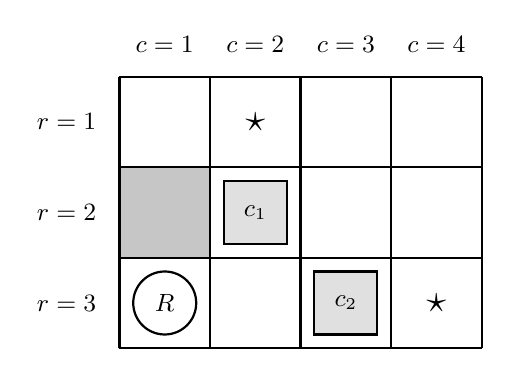
\begin{tikzpicture}[scale=1.15, every node/.style={font=\small}]
  \fill[gray!45] (0,1) rectangle (1,2);
  \draw[step=1cm, black, thick] (0,0) grid (4,3);
  \node[font=\Large] at (1.5,2.5) {$\star$};
  \node[font=\Large] at (3.5,0.5) {$\star$};
  \node[draw, thick, fill=black!12, minimum size=8mm] at (1.5,1.5) {$c_1$};
  \node[draw, thick, fill=black!12, minimum size=8mm] at (2.5,0.5) {$c_2$};
  \node[draw, thick, circle, fill=white, minimum size=8mm] at (0.5,0.5) {$R$};
  \foreach \c in {1,2,3,4} \node at (\c-0.5,3.35) {$c=\c$};
  \foreach \r/\y in {1/2.5,2/1.5,3/0.5} \node[left] at (-0.15,\y) {$r=\r$};
\end{tikzpicture}
\end{figure}
\noindent
$R$ is the robot at $(3,1)$; $c_1$ and $c_2$ are crates at $(2,2)$ and $(3,3)$;
the two $\star$ cells $(1,2)$ and $(3,4)$ are the marked squares; the shaded cell $(2,1)$ is
the obstacle.
\begin{enumerate}
\clearpage
\item \points[2] Explain why a simple search over the robot's grid position alone (i.e., one
that treats a state as just the cell the robot occupies) would be \emph{insufficient} for this
problem. Give a specific example.
\begin{solution}
The robot's cell does not determine either the goal test or the available actions, because the
crates move too.
\\~\\
Concretely, consider the robot at $(3,2)$. If $c_1$ is still at $(2,2)$, then moving \texttt{up}
is a push that sends $c_1$ to $(1,2)$; if $c_1$ has already been moved to $(1,2)$, the very same
\texttt{up} move from the very same cell is an ordinary relocation. One ``state'' $(3,2)$ therefore
has two different successor sets. Equally, the position $(3,2)$ tells us nothing about whether the
task is finished --- the goal is a property of the crates, not the robot.
\\~\\
Accept any answer that identifies that crate configuration must be part of the state. A strong
answer may also note that some pushes are \emph{irreversible}: pushing a crate into a corner or
against the obstacle makes the task unsolvable forever after, so the search must be able to
distinguish those configurations.
\end{solution}
\vspace{2cm}
\item \points[8] Model this as a search problem by filling in each component below. You may not need all of the boxes.
  \begin{enumerate}
  \item \points[2] Each state is a tuple,
  \[\left(\ansbox[2.4cm]{$p_R$},\ansbox[2.4cm]{$p_1$},\ansbox[2.4cm]{$p_2$},\ansbox[2.4cm]{},\ansbox[2.4cm]{} \right),\]
  where: \\[2mm]
  \begin{itemize}
      \item \; \ansnt{$p_R$: the cell $(r,c)$ occupied by the robot} \\[5mm]
      \item \; \ansnt{$p_1$: the cell occupied by crate $c_1$} \\~\\
      \item \; \ansnt{$p_2$: the cell occupied by crate $c_2$} \\~\\
      \item \; \ansnt{(unused)} \\~\\
      \item \; \ansnt{(unused)}
  \end{itemize}
  \begin{solution}
  Only three components are needed; the last two boxes are left blank.
  \\~\\
  An equally good answer replaces $p_1,p_2$ with the unordered \emph{set} $\{p_1,p_2\}$ of occupied
  crate cells, since the crates are interchangeable --- this halves the state space and is worth
  full marks.
  \\~\\
  Marking scheme:
  \begin{itemize}
      \item 2 marks for a minimal correct state: robot cell plus the crate configuration
      \item 1.5 marks for a slightly redundant but correct state. E.g., also stored the move count or the path taken
      \item 0-1 marks for a state that omits the crates, or that stores only ``how many crates are done'' rather than where they are
  \end{itemize}
  \end{solution}
  \item \points[1] Write the initial state using your representation.
    \[s_0 = \left(\ansbox[2.4cm]{$(3,1)$},\ansbox[2.4cm]{$(2,2)$},\ansbox[2.4cm]{$(3,3)$},\ansbox[2.4cm]{},\ansbox[2.4cm]{}\right)\]
  \item \points[1] Describe which states are goal states using your representation.
  % \vspace{100pt}
  \begin{solution}
      Any state with $\{p_1,p_2\} = \{(1,2),(3,4)\}$, with $p_R$ arbitrary. Note that both assignments count: $p_1=(1,2), p_2=(3,4)$ and $p_1=(3,4), p_2=(1,2)$ are both goals.
  \end{solution}
  \item \points[2] For a generic state $s$, describe how to determine its successors
        (i.e., the states reachable via a single action).
  % \vspace{100pt}
  \begin{solution}
      For each of the four directions $\delta \in \{\texttt{up},\texttt{down},\texttt{left},\texttt{right}\}$, let $n = p_R + \delta$ be the neighbouring cell and $b = p_R + 2\delta$ the cell beyond it.
      \begin{itemize}
        \item If $n$ is off the grid or is the obstacle $(2,1)$: no successor.
        \item If $n$ is empty: successor is the same state with $p_R \leftarrow n$.
        \item If $n$ holds a crate: the move is legal only if $b$ is on the grid, is not the obstacle, and does not hold the other crate. If so, the successor sets $p_R \leftarrow n$ and moves that crate to $b$; otherwise there is no successor in that direction.
      \end{itemize}
      Every successor has cost $1$.
      \\~\\
      Marking scheme: 1 mark for the ordinary-move case and the grid/obstacle bounds; 1 mark for correct push semantics (checking the cell \emph{beyond} the crate, including the other crate blocking it). Only 1 mark total if the student describes only the robot's movement and never updates the crate positions.
  \end{solution}
  \item \points[2] Describe an admissible heuristic for this problem.
        Explain in one or two sentences why your heuristic is admissible.
  % \vspace{80pt}
  \begin{solution}
  One helpful heuristic: for each crate, take the Manhattan distance to the nearer marked square, and sum the two. This is admissible because each crate must be pushed at least once per unit of Manhattan distance, each push costs $1$, and the robot's own repositioning moves only add further cost --- so the sum is a lower bound on the true remaining cost. (It also ignores the obstacle and the crates blocking each other, which can only reduce the estimate.)
  \\~\\
  At $s_0$ this gives $h(s_0) = 1 + 1 = 2$, whereas the optimal solution costs $4$:
  $\texttt{right}$, $\texttt{up}$ (push $c_1$ to $(1,2)$), $\texttt{down}$, $\texttt{right}$ (push $c_2$ to $(3,4)$).
  \\~\\
  Any technically admissible heuristic is also accepted. E.g. $h(x)=0$ is not very helpful but technically admissible. Do \emph{not} give marks for the robot's own distance to a crate or to a target, which is not a lower bound on the remaining cost in any useful sense; give at most 1 mark if the justification is missing.
  \end{solution}
  \end{enumerate}
\end{enumerate}
\clearpage
\begin{center}
    \textit{(extra space)}
\end{center}
\clearpage
%% ============================================================
\section{\points[8] Markov Decision Processes (Advanced)}
\subsection{\points[8] Modelling}
A maintenance depot keeps spare actuators on a shelf that holds at most $3$ units.
At the start of each week the depot observes how many units $s$ are on the shelf and decides
how many units $a$ to order; an order arrives immediately, and the shelf capacity may not be
exceeded, so $0 \le a \le 3-s$.
\medskip\noindent
Demand $D$ then arrives over the course of the week, independently each week, with
\[
\textsf{pr}[D=0]=0.2, \qquad \textsf{pr}[D=1]=0.5, \qquad \textsf{pr}[D=2]=0.3.
\]
Each unit of demand that can be met from the shelf is filled; any excess demand is lost (the
technician sources that unit elsewhere). Whatever remains on the shelf at the end of the week
carries over to the next week.
\medskip\noindent
The rewards for a week are as follows:
\begin{itemize}
  \item $+6$ for each unit supplied from the shelf
  \item $-2$ for each unit ordered
  \item $-1$ for each unit still on the shelf at the end of the week (storage)
  \item $-5$ for each unit of demand that could not be met
\end{itemize}
\medskip\noindent
The depot wants to maximise its total expected reward over many weeks.
\begin{enumerate}
\item \points[1] Assume each state is the number of units on the shelf at the \emph{start} of a
week, before ordering. Define the state space $\mathcal{S}$ for this MDP by providing the list of
all the states.
\\~\\
$\mathcal{S} = \left\lbrace \ansbox[3cm]{$0$}, \ansbox[3cm]{$1$}, \ansbox[3cm]{$2$}, \ansbox[3cm]{$3$} \right\rbrace$
\vspace{60pt}
\item \points[3] Write out the full transition function $p(s' \mid s, a)$ for the state
$s = 1$ under each of the actions available in that state.
Present your answer as a table.
\renewcommand{\arraystretch}{1.9}
\begin{table}[H]
\centering
\begin{tabular}{|l|l|c|}
\hline
Action & Next state $s'$ & $p(s' \mid s, a)$ \\\hline
\multirow{2}{*}{$a=0$}
  & $s'=1$ & \ansnt{$0.2$} \\\cline{2-3}
  & $s'=0$ & \ansnt{$0.8$} \\\hline
\multirow{3}{*}{$a=1$}
  & $s'=2$ & \ansnt{$0.2$} \\\cline{2-3}
  & $s'=1$ & \ansnt{$0.5$} \\\cline{2-3}
  & $s'=0$ & \ansnt{$0.3$} \\\hline
\multirow{3}{*}{$a=2$}
  & $s'=3$ & \ansnt{$0.2$} \\\cline{2-3}
  & $s'=2$ & \ansnt{$0.5$} \\\cline{2-3}
  & $s'=1$ & \ansnt{$0.3$} \\\hline
\end{tabular}
\end{table}
\begin{solution}
Write $y = s+a$ for the units on hand after the order arrives; then
$s' = \max(0,\, y - D)$.
\\~\\
For $s=1$ the available actions are $a \in \{0,1,2\}$.
\begin{itemize}
  \item $a=0 \Rightarrow y=1$: $D=0$ leaves $s'=1$ (prob $0.2$); $D=1$ and $D=2$ both leave $s'=0$, so $\textsf{pr}[s'=0] = 0.5+0.3 = 0.8$. Note that the two demand outcomes \emph{merge}, because demand beyond the shelf is lost rather than backordered.
  \item $a=1 \Rightarrow y=2$: $s' = 2,1,0$ with probabilities $0.2, 0.5, 0.3$.
  \item $a=2 \Rightarrow y=3$: $s' = 3,2,1$ with probabilities $0.2, 0.5, 0.3$.
\end{itemize}
Marking scheme: 1 mark per action. The most common error is to give $a=0$ four outcomes or to
assign $\textsf{pr}[s'=0]=0.5$, missing that lost demand collapses $D=1$ and $D=2$ onto the same
next state.
\end{solution}
\clearpage
\item \points[2] A student proposes the following policy:
\begin{quote}
  \emph{``Never order. Ordering always costs money, and any demand we cannot fill is simply
  sourced elsewhere.''}
\end{quote}
Give a concrete argument (using the reward structure and the demand distribution) for why
this policy may \emph{not} be optimal.
\begin{solution}
For marking: look for a comparison of expected rewards between ordering and not ordering in
some state, using the demand distribution.
\\~\\
Under this policy the shelf empties and stays empty, so consider $s=0$.
\\~\\
With $a=0$ nothing can be supplied and every unit of demand is lost. The expected lost demand is
$\mathbb{E}[D] = 0(0.2)+1(0.5)+2(0.3) = 1.1$, so the expected weekly reward is
\[
0 - 5(1.1) = -5.5.
\]
With $a=1$ the depot pays $-2$ to order one unit, then supplies $\min(1,D)$ units and loses
$\max(0,D-1)$:
\[
\mathbb{E}[\text{supplied}] = 0(0.2)+1(0.5)+1(0.3) = 0.8, \qquad
\mathbb{E}[\text{lost}] = 0(0.2)+0(0.5)+1(0.3) = 0.3,
\]
\[
\mathbb{E}[\text{held}] = 1(0.2)+0(0.5)+0(0.3) = 0.2,
\]
\[
\mathbb{E}[r \mid s=0,a=1] = -2 + 6(0.8) - 5(0.3) - 1(0.2) = -2 + 4.8 - 1.5 - 0.2 = 1.1.
\]
Since $1.1 > -5.5$, ordering is better than not ordering \emph{even for a single week}, before
any consideration of future value. The student's argument ignores the $-5$ lost-sale penalty,
which is larger than the $-2$ order cost.
\end{solution}
\vspace{60pt}
\item \points[2] A second student claims:
\begin{quote}
  \emph{``Then the depot should always order up to the full capacity of $3$, so that it is never
  caught short.''}
\end{quote}
Give a concrete counter-argument showing a state in which this is \emph{not} optimal.
Your answer should reference specific states and expected rewards.
% \vspace{80pt}
\begin{solution}
For marking: look that they compared the expected rewards of two actions in one state correctly.
\\~\\
Consider $s=2$ and compare $a=0$ (do nothing) with $a=1$ (top up to $3$).
\\~\\
With $y=2$ units on hand, demand is never more than $2$, so nothing is ever lost:
\[
\mathbb{E}[\text{supplied}] = 0(0.2)+1(0.5)+2(0.3) = 1.1, \qquad
\mathbb{E}[\text{held}] = 2(0.2)+1(0.5)+0(0.3) = 0.9,
\]
\[
\mathbb{E}[r \mid s=2,a=0] = 6(1.1) - 1(0.9) = 6.6 - 0.9 = 5.7.
\]
With $y=3$ units on hand the expected units supplied is unchanged at $1.1$ --- the third unit can
never be sold, because $D \le 2$ --- while the depot pays for it and stores it:
\[
\mathbb{E}[\text{held}] = 3(0.2)+2(0.5)+1(0.3) = 1.9,
\]
\[
\mathbb{E}[r \mid s=2,a=1] = -2 + 6(1.1) - 1(1.9) = -2 + 6.6 - 1.9 = 2.7.
\]
So $5.7 > 2.7$: at $s=2$ the third unit is strictly wasteful. It cannot raise this week's revenue,
it costs $-2$ to buy and an extra $-1$ to store, and it only defers a purchase the depot could
make later anyway.
\\~\\
The two students bracket the truth: the optimal policy orders when the shelf is nearly empty and
stops short of capacity. (For reference, solving this MDP with $\gamma = 0.9$ gives the order
policy $a^*(0)=2$, $a^*(1)=1$, $a^*(2)=0$, $a^*(3)=0$ --- i.e.\ ``order up to $2$ units on hand''.
Students are not expected to compute this.)
\end{solution}
\end{enumerate}
